%%%%%%%%%%%%%%%%%%%%%%%%%%%%%%%%%%%%%%%%%
% Calculus Fight Club (CFC) Handbook
% By: Ryan Grove
%%%%%%%%%%%%%%%%%%%%%%%%%%%%%%%%%%%%%%%%%

%----------------------------------------------------------------------------------------
%	PACKAGES AND OTHER DOCUMENT CONFIGURATIONS
%----------------------------------------------------------------------------------------

\documentclass[paper=a4, fontsize=11pt]{scrartcl} % A4 paper and 11pt font size

\usepackage[T1]{fontenc} % Use 8-bit encoding that has 256 glyphs
\usepackage{fourier} % Use the Adobe Utopia font for the document - comment this line to return to the LaTeX default
\usepackage[english]{babel} % English language/hyphenation
\usepackage{amsmath,amsfonts,amsthm} % Math packages

\usepackage{lipsum} % Used for inserting dummy 'Lorem ipsum' text into the template

\usepackage{sectsty} % Allows customizing section commands
\allsectionsfont{\centering \normalfont\scshape} % Make all sections centered, the default font and small caps

\usepackage{fancyhdr} % Custom headers and footers
\pagestyle{fancyplain} % Makes all pages in the document conform to the custom headers and footers
\fancyhead{} % No page header - if you want one, create it in the same way as the footers below
\fancyfoot[L]{} % Empty left footer
\fancyfoot[C]{} % Empty center footer
%\fancyfoot[R]{\thepage} % Page numbering for right footer
\renewcommand{\headrulewidth}{0pt} % Remove header underlines
\renewcommand{\footrulewidth}{0pt} % Remove footer underlines
\setlength{\headheight}{13.6pt} % Customize the height of the header

\numberwithin{equation}{section} % Number equations within sections (i.e. 1.1, 1.2, 2.1, 2.2 instead of 1, 2, 3, 4)
\numberwithin{figure}{section} % Number figures within sections (i.e. 1.1, 1.2, 2.1, 2.2 instead of 1, 2, 3, 4)
\numberwithin{table}{section} % Number tables within sections (i.e. 1.1, 1.2, 2.1, 2.2 instead of 1, 2, 3, 4)

\setlength\parindent{0pt} % Removes all indentation from paragraphs - comment this line for an assignment with lots of text

\usepackage{lastpage}
\usepackage{fancyhdr}
\usepackage{listings}
\usepackage{graphicx}
\cfoot{\thepage\ of \pageref{LastPage}}

%----------------------------------------------------------------------------------------
%	TITLE SECTION
%----------------------------------------------------------------------------------------

\newcommand{\horrule}[1]{\rule{\linewidth}{#1}} % Create horizontal rule command with 1 argument of height

\title{	
\normalfont \normalsize 
\textsc{Clemson University - MATH1020, MATH1060, MATH1080 \& MATH2070} \\ [25pt] % Your name, university, class
\horrule{0.5pt} \\[0.4cm] % Thin top horizontal rule
\huge Calculus Fight Club (CFC) Handbook \\ % The assignment title
\horrule{2pt} \\[0.5cm] % Thick bottom horizontal rule
}

\author{Last Updated:} % The due date

\date{\normalsize March 8th, 2017} % A custom date

\begin{document}

\maketitle % Print the title

\begin{center}
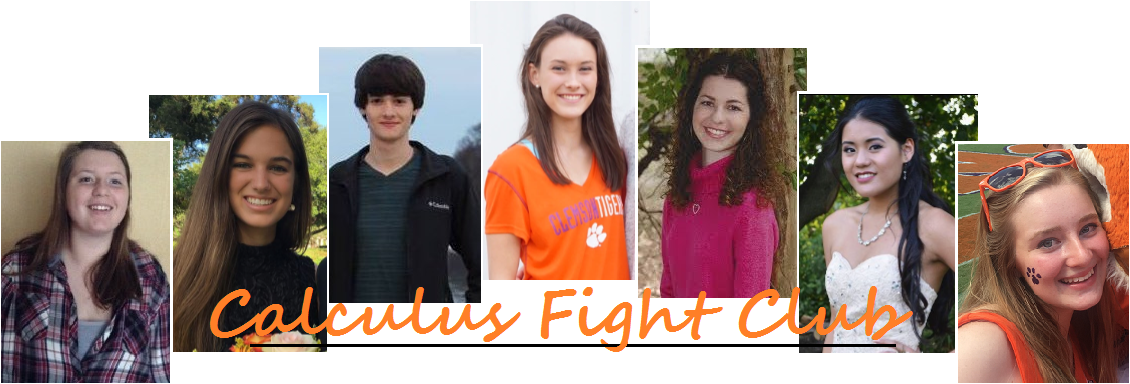
\includegraphics[scale=.5]{cfc.png}
\end{center}


%----------------------------------------------------------------------------------------
%	Purpose
%----------------------------------------------------------------------------------------

\section*{\textbf{Purpose:}}

Created in 2015 by Ryan Grove, Calculus Fight Club is taught by students currently enrolled in a MATH1020, MATH1060, MATH1080 or MATH2070 class (\textit{as well as PAL leaders for these classes}) at Clemson University that volunteer their time to help any students taking these classes prepare for upcoming tests by going over selected problems from previous semesters' exams on the Monday night of the week of a test. \\

Calculus Fight Club works closely with the MATH1020, MATH1060, MATH1080 and MATH2070 course coordinators in order to find teachers for each Calculus Fight Club, confirm which material will be relevant to go over for each test, and to get the word out so that students in those classes know about our event.  On average, Calculus Fight Club provides around 400-500 students per event with a chance to spend a night studying calculus with their peers in an environment that is entirely led by their peers.  The current head coordinator of Calculus Fight Club is AJ Miller (\textit{ajm4@g.clemson.edu}).  The current coordinators are (pictured left to right):  Hannah Berg (\textit{for MATH1080}), Addie Stone (\textit{for MATH1020}), Mary Guest (\textit{for MATH2070}), Polly Payne (\textit{for MATH1060}), Amelia Casella (\textit{for MATH2070}) and Allison Kaczmarek (\textit{for MATH1080}).

%----------------------------------------------------------------------------------------
%	Leader Responsibilities
%----------------------------------------------------------------------------------------

\section*{\textbf{CFC Coordinator Responsibilities:}}

The responsibilities of being a CFC Coordinator include: 

\begin{enumerate}
\item \textbf{Picking the times of the CFC \& deciding how many rooms you'll need:} These are both fairly easy because you can use previous years as a guide (\textit{i.e. The Monday before each test from 9pm-midnight seemed to work fine while I was in charge and having the entire first and second floor of Martin M as well as the auditorium plus random rooms in Daniel seems to be enough rooms for the amount of students we see coming to CFC}).  You also need to let all of the course coordinators know the date and time of each CFC.
\item \textbf{Reserving the rooms \& finding student teachers:} Coordinators will be allowed to make reservations in the Mathematical Sciences Department by contacting April Haynes \\ (\textit{ahayne@clemson.edu}), but finding student teachers is very much up to you all.  The best way we found to do this in the past is to ask the course coordinators to e-mail ALL instructors and ask them to ask some of their better students if they are interested.
\item \textbf{Figuring out which material is relevant:} This is just a mixture of looking at the old tests and talking to the course coordinators.  Then, you would e-mail (\textbf{please see my old e-mail below}) your student teachers and tell them what the plan is! Finally, typically what is done is that you would print out as many copies of the tests as you have found students to teach, and then give them to your student teachers as they arrive on the night of CFC.
\item \textbf{Teaching the student teachers how to teach:} It is a good idea to meet about an hour and a half early on nights of CFC to teach the new teachers good teaching practices and how to deal with a full room of students.
\item \textbf{Communicating frequently with each other:} As there are coordinators for every class covered, it is important that all CFC coordinators stay in contact with each other.  We typically just use e-mails to do this and try to figure out everything for a coming CFC at least 2 weeks in advance, as well as carbon copy each other on the report after each CFC.
\item \textbf{Finding your successor:} And, alas, eventually you will either have to graduate or not have enough time in your schedule to dedicate to CFC and you will need to work on finding your successor.  When doing this, you should definitely try to highlight all the positive aspects that they might not see right away from leading such a large community service-oriented organization!
\end{enumerate}

Overall, I would expect that you would spend about 20-30 hours a semester (between e-mails, meeting with course coordinators, teaching at CFC, etc.) on CFC from my own personal experience, so keep that in mind as you decide if you want to be a leader of CFC.  Also, the Mathematical Science department as well as the people in charge of PAL work very closely with us and we have had much good communication and sharing of ideas and students throughout the years.  Therefore, one of the biggest selling points we use for finding teachers of CFC is that CFC gives you a much higher chance of becoming a PAL leader (\textit{as well as seeing if you would even like becoming a PAL leader}). 

\section*{\textbf{Calculus Fight Club Checklist:}}
A checklist of things that need done for every CFC is described here.  The current head coordinator is AJ Miller (\textit{ajm4@g.clemson.edu}), so please include him in on all of your e-mails to course coordinators as well as student teachers.
\begin{itemize}
\item As students contact you saying that they'd like to participate in CFC, send them an e-mail back saying "thank you for your interest in becoming a CFC leader" as well as a guess as to when you will be in touch with them with more information!
\item No later than 1 week before each CFC, e-mail the course coordinator details about each CFC including: date, time, location for your specific class, and point of contact.  Also, ask the course coordinator when he/she can meet to go over the material with you.  Please copy the current CFC head coordinator on these e-mails.
\item Once you meet with the course coordinator, create examples of like questions that students could work on in CFC and then create an e-mail in which you explain to your student leaders what the course coordinator has decided to have you over for the upcoming CFC, as well as any examples you have added.  Please copy the current CFC head coordinator on these e-mails.
\item Prepare a packet for each student leader that contains all of the material that they are supposed to teach at CFC as well as all of the examples you have included.
\item No later than one day after each CFC, send the course coordinators an e-mail that says how many people came, how it went overall, suggestions for improvement, as well as if you require more student teachers or more rooms to teach in.  Please copy ALL CFC coordiantors on this e-mail.
\end{itemize}

Whoever is reserving the rooms is in charge of contacting April Haynes (\textit{ahayne@clemson.edu}) at least 2 weeks before every CFC and letting her know which all rooms need reserved.

\section*{\textbf{Contact Information:}}
\begin{itemize}
\item \textbf{Head Coordinator:} AJ Miller (\textit{ajm4@g.clemson.edu})
\item \textbf{MATH1020 Coordinator:} Addie Stone (\textit{adstone@g.clemson.edu})
\item \textbf{MATH1060 Coordinator:} Polly Payne (\textit{pollyp@g.clemson.edu})
\item \textbf{MATH1080 Coordinator:} Hannah Berg (\textit{hnberg@clemson.edu})
\item \textbf{MATH1080 Coordinator:} Allison Kaczmarek (\textit{rrgrove6@gmail.com})
\item \textbf{MATH2070 Coordinator:} Mary Guest (\textit{mdguest@g.clemson.edu})
\item \textbf{MATH2070 Coordinator:} Amelia Casella (\textit{awcasel@g.clemson.edu})
\item \textbf{Founder:} Ryan Grove (\textit{rrgrove6@gmail.com})
\item \textbf{Master of the Keys:} April Haynes (\textit{ahayne@clemson.edu})
\end{itemize}

\section*{\textbf{Sample E-mail to CFC Teachers from CFC Leader:}}
Student Teachers of Calculus Fight Club, \\

Thank you all for helping me out during this installment of Calculus Fight Club for the Final Exam!  The official date and time is 9pm-midnight on Thursday, April 21st. Basically my plan is that I put two of you in each room [we have 4 rooms for MATH1080 (Martin M201,M202,M203,M205)] and that way when I'm rotating around there can always be teaching or helping going on!  Here are links to all of the solutions to the material you will be teaching: 
\begin{lstlisting}
https://mthsc.clemson.edu/ug_course_pages/view_course_page.py?course_id=8
\end{lstlisting}

If this is your first time teaching, you'll be amazed at how well you will understand the material after you have to teach it/people ask lots of questions that you have to really think about!  All student teachers will meet with me 1 hour before Calculus Fight Club (so 8pm in MartinM202) to discuss any questions/concerns you any have about teaching, the material, and/or how to get the students engaged and asking questions! \\

The teaching teams will be as follows: \\
John and Stephen (Martin M205) \\
Annie and Michael (Martin M201) \\
Jennah, James, Daniel, and AJ (Martin M203) \\
Aaron and Matthew (Martin M202) \\
Polly (Martin M101) \\

Please e-mail your teaching partner(s) and discuss how you would like to split up the following material: (Note: TEACH means you teach that problem step-by-step at the board slowly and clearly, whereas DO means you have the students do that problem in groups then go over it on the board once the majority of the groups finish). \\

For MATH1080: \\

1st Section (40 mins): \\
TEACH Spring'15 Test $\#  2$ Question $\# 9$ \\
TEACH Spring'15 Test $\# 2$ Question $\# 10$ \\
DO Fall'15 Test $\# 2$ Question $\# 1$ \\
DO Fall'15 Test $\# 2$ Question $\# 5$ \\

2nd Section (40 mins): \\
TEACH Fall'15 Test $\# 2$ Question $\# 3$ \\
DO Spring'15 Test $\# 3$ Question $\# 1$ \\

3rd Section (40 mins): \\
DO Spring15 Test $\# 2$ Question $\# 4$ \\
DO Fall'15 Test $\# 2$ Question $\# 6$ \\

4th Section (60 mins): \\
Ask for any questions on anything in MATH1080 for the last hour. \\

%----------------------------------------------------------------------------------------

\end{document}